\section{Proposed Approach} \label{sec:approach}
Il dataset prevede 60.000 campioni di training e 10.000 di test, è stato però necessario ridurre il numero di sample per il training set così da avere delle tempistiche ragionevoli per effettuare l'addestramento delle reti. Sono quindi stati estratti i primi 5.000 sample per il training e di conseguenza la dimensione del test set è stata portata a 1.000 campioni. Come mostrato nelle Figure \ref{fig2:train_sample_distribution} e \ref{fig3:test_sample_distribution} la distribuzione delle etichette rimane comunque bilanciata sia nel training che nel test set.
\begin{figure}[!hbt]
    \centering
    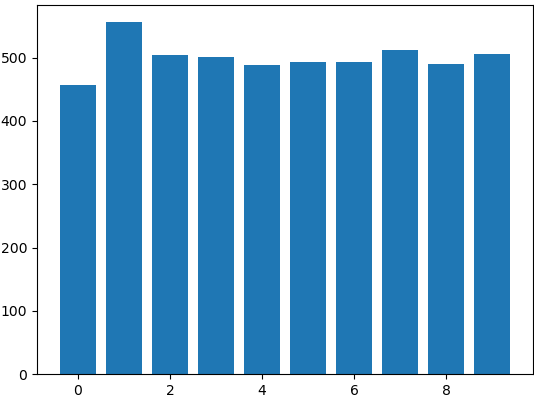
\includegraphics[width=\columnwidth]{images/train_sample_distribution2.png}
    \caption{Distribuzione label training set dopo la riduzione del dataset}
    \label{fig2:train_sample_distribution}
\end{figure}

\begin{figure}[!hbt]
    \centering
    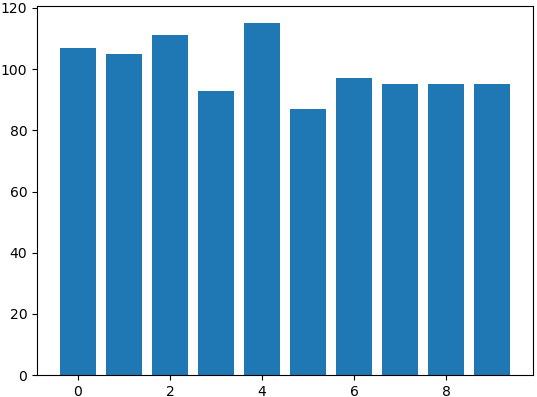
\includegraphics[width=\columnwidth]{images/test_sample_distribution2.png}
    \caption{Distribuzione label test set dopo la riduzione del dataset}
    \label{fig3:test_sample_distribution}
\end{figure}


\subsection*{CustomNet}
L'architettura (Figura \ref{fig4:custom_net_architecture}) è costituita da tre blocchi convoluzionali, i primi due del tutto identici fra loro, il terzo è stato leggermente modificato rispetto  ai precedenti:
\begin{enumerate}
\item \textbf{Convolutiona layer}\\
\-\ input ch: 1\\ \-\ out ch: 32\\ \-\ kernel_size: $3\times3$\\ \-\ stride: 1\\ \-\ padding: 1
\item \textbf{Batch Normalization}
\item \textbf{ReLU}
\item \textbf{Max Pooling 2D}\\
\-\ kernel size: $2\times2$\\ \-\ stride: 2

\item \textbf{Convolutional layer}\\
\-\ input ch: 32\\ \-\ out ch: 64\\ \-\ kernel_size: $3\times3$\\ \-\ stride: 1\\ \-\ padding: 1
\item \textbf{Batch Normalization}
\item \textbf{ReLU}
\item \textbf{Max Pooling 2D}\\
\-\ kernel size: $2\times2$\\ \-\ stride: 2

\item \textbf{Convolutional layer}\\
\-\ input ch: 64\\ \-\ out ch: 128\\ \-\ kernel_size: $3\times3$\\ \-\ stride: 1\\ \-\ padding: 1
\item \textbf{Batch Normalization}
\item \textbf{ReLU}
\item \textbf{Dropout}\\
\-\ probability: 0.5
\item \textbf{Fully connected}\\
\-\ in size: 6272\\ \-\ out size: 10
\end{enumerate}
\begin{figure}[!hbt]
    \centering
    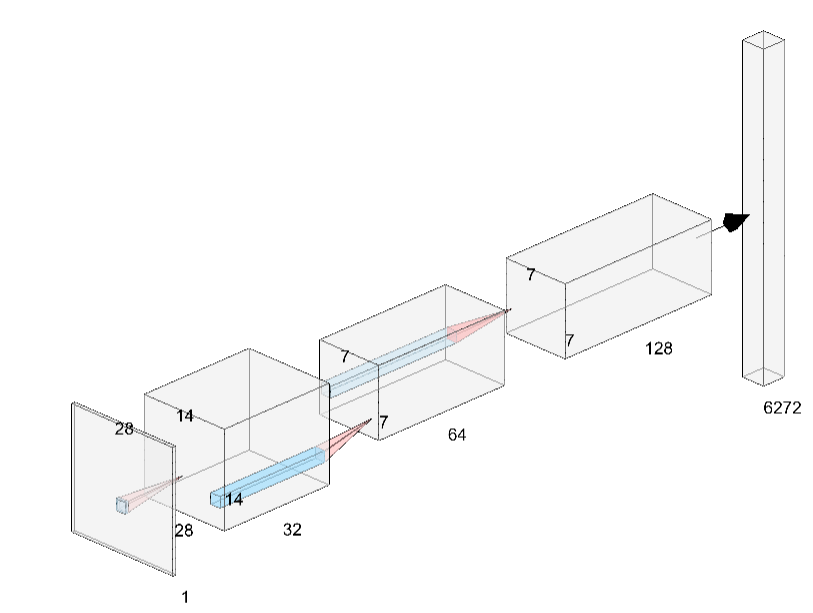
\includegraphics[width=\columnwidth]{images/CustomNetArchitecture.png}
    \caption{Architettura CustomNet}
    \label{fig4:custom_net_architecture}
\end{figure}
In tutti i blocchi la dimensione del kernel è $3\times3$, impilare layer convoluzionali con kernel di dimensioni ridotte consente di avere una maggior espressività delle feature ed un minor numero di parametri rispetto ad un unico layer convoluzionale avente un kernel di dimensioni maggiori. \`{E} stato sempre applicato il padding same  così da non ridurre la dimensione del tensore in input al blocco successivo a seguito della convoluzione. Successivamente è stato inserito il layer di batch normalization così da normalizzare l'output della convoluzione che poi andrà in input alla funzione di attivazione. ReLU (Rectified Linear Unit) è una funzione non lineare definita come:
$$f(x) = max(0,x)$$
Nei primi due blocchi è stato applicato un max pooling, questo consente di ottenere una statistica sommaria degli output del layer precedente nell'intorno del pixel e una rappresentazione invariante a piccole traslazioni dell'input. I parametri impostati per il pooling dimezzano la dimensione del volume in ingresso. In Figura \ref{fig4:custom_net_architecture} è mostrato un esempio di applicazione di max pooling.
\begin{figure}[!hbt]
    \centering
    \includegraphics[width=\columnwidth]{images/MaxPoolSample2.png}
    \caption{Applicazione max pooling con kernel $2\times2$ e stride 2}
    \label{fig5:max_pooling}
\end{figure}
Nell'ultimo blocco al posto del max pooling è stato introdotto  un layer di dropout \cite{srivastava2014dropout} per effettuare la regolarizzazione e quindi prevenire l'overfitting.Il dropout è una tecnica di regolarizzazione estremamente efficace che consiste nel mantenere un neurone attivo con probabilità $p$, questo si traduce in fase di training con l'eliminazione di alcune connessioni randomicamente in base a $p$. Così facendo la rete utilizza un numero di parametri inferiore e non sapendo a priori quali connessioni verranno inibite è costretta ad apprendere i concetti veramente importanti. Infine vi è il layer fully connected che produce in uscita la predizione, chiaramente è stato necessario effettuare precedentemente la vettorializzazione del tensore.
\subsection*{Resnet-18}
Essendo Resnet-18 un'architettura fondamentale non è stato necessario implementarla da zero, tuttavia la struttura è stata modificata in alcuni punti per adattarla al task in questione. \`{E} stato sostituito il primo layer convoluzionale dato che questo prende in input immagini RGB, quindi aventi 3 canali. Il nuovo layer, sempre convoluzionale, ha gli stessi parametri dell'originale fatta eccezione per la dimensione dell'input che passa da 3 a 1. A valle della rete l'ultimo layer fully connected è stato modificato per avere l'uscita di dimensione pari al numero delle classi, cioè 10.\par
\`{E} stata scelta questa rete essendo uno standard attuale che  rappresenta la backbone delle moderne reti neurali, è stato inoltre il progetto vincitore nel 2015 di ILSVRC \cite{ILSVRC15} (ImageNet Large Scale Visual Recognition Challenge).
\begin{figure}[!hbt]
    \centering
    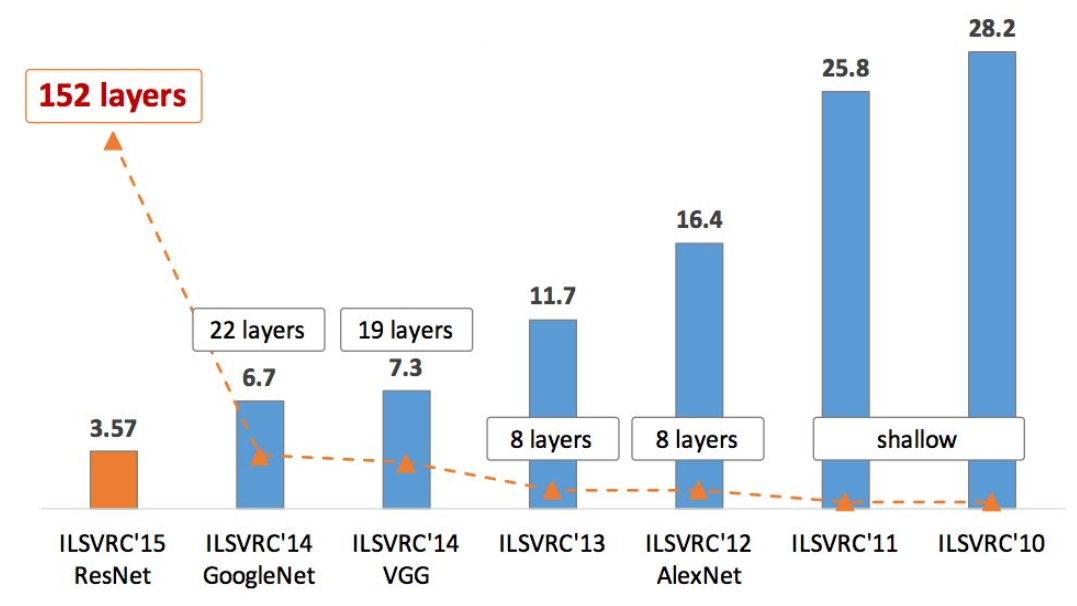
\includegraphics[width=\columnwidth]{images/ilsvrc_winners.png}
    \caption{Vincitori di ILSVRC dal 2010 al 2015}
    \label{fig6:ILSVRC2015}
\end{figure}\par
L'elemento caratterizzante di questa rete sono i residual block: questi consento al gradiente di propagarsi all'indietro nella rete senza essere alterato cosi da scongiurare il problema del \textit{vanishing gradient}.




  